\documentclass{article}

\usepackage{amsmath,amsfonts,graphicx,fullpage,comment,verbatim}

\newcommand{\HRule}{\rule{\linewidth}{0.5mm}}
\begin{document}

\begin{titlepage}
 
\begin{center}
 
\textsc{\LARGE Homework 2}\\[1.5cm] 

\textsc{\Large Computational Math}\\[0.5cm]
 
 
\HRule \\[2cm]
 
% Author and supervisor
\begin{minipage}{0.4\textwidth}
\begin{flushleft} \large
\emph{Author:}\\
Mikola Lysenko
\end{flushleft}
\end{minipage}
 
\vfill
 
% Bottom of the page
{\large \today}
 
\end{center}
 
\end{titlepage}


\paragraph{1}

\subparagraph{a}

I checked the exactness condition for the given $u$ using sympy and a Python script:

\begin{verbatim}
from sympy import *;

def uexact(x):
	return exp(sin(x)) * exp(cos(x));
	
def q1(x):
	return sin(x) * cos(x);
	
def q2(x):
	return -2 * cos(x)**4 + cos(x)**3 + (8 + 3 * sin(x)) * cos(x)**2 - (1 + sin(x)) * cos(x);

u = uexact(x);
ux = diff(u, x);
uxx = diff(ux, x);
uxxx = diff(uxx, x);
print trigsimp(simplify(uxxx + q1(x) * uxx + q2(x) * u(x) - 3 * exp(sin(x)) * exp(cos(x)))) == 0;
\end{verbatim}

By inspection, it should be clear that if uexact is an exact solution for the ode, then it ought to print out True; which is exactly what happens, and so the exactness condition is satisified.

\subparagraph{b}

Based on class discussion, pick 
\[u(x) = \sum \limits_{j=0}^N w_j C_j(x) \]
Where
\[ C_j(x) = \frac{1}{N} \sin \left[ \frac{N (x - x_j)}{2} \right] \cot \left[ \frac{(x - x_j)}{2} \right] \]
In the interval $[-\pi, \pi)$.  Now observe that $C_j$ has a nice, finite Fourier series expansion, (assuming $N$ is divisible by 4):
\[ C_j(x) = \frac{1}{N} \left( -\frac{1}{2} e^{\pm i N/2 (x - x_j)} + \sum \limits_{k=-N/2}^{N/2} e^{i k (\pi + x - x_j)} \right) \]
Differentiating $C_j$, $d$-times is equivalent to applying the Fourier multiplier $(ik)^d$, and so:
\[ \partial^d_x C_j(x) = \frac{1}{N} \left( -\frac{(iN)^d}{2^{d+1}} e^{\pm i N/2 (x - x_j)} + \sum \limits_{k=-N/2}^{N/2} (ik)^d e^{i k (\pi + x - x_j)} \right)
\]
To compute the weights for the differentiation matrix, $D^d$, we need need to compute:
\[ D^d_{p,q} = \langle \partial^d_x C_p , C_q \rangle \]
But due to the cancellative properties of sinc interpolation, this reduces to:
\[ D^d_{p,q} = \partial^d_x C_p(x_q) \]
Pick $d=3$ and we are done.

\subparagraph{c}
We compute the differentiation matrix numerically using the fast fourier transform.  Here is some MATLAB code I wrote to do this:

\begin{verbatim}
function [ D ] = sinc_d( N, d )
  k = [0:(N/2) (1-N/2):-1];
  ch = ones(1,N);
  chd = (i * k).^d .* ch;
  dc = real(ifft(chd));
  D = toeplitz(dc, dc([1 N:-1:2]));
\end{verbatim}

Once we have the matrix computed, we just solve for the solution using the vanilla Galerkin method for sinc functions:

\begin{verbatim}
x = (0:N-1) * 2 * pi / N;
D2 = sinc_d(N, 2);
D3 = sinc_d(N, 3);
s = sin(x);
c = cos(x);
q1 = s .* c;
q2 = -2.*c.^4 + c.^3 + (8. + 3. * s) .* c.^2 - (1. + s) .* c;
f = 3. * exp(s) .* exp(c);
L = D3 + diag(q1) * D2 + diag(q2);
u = L \ f';
\end{verbatim}

Here is a plot of the exact solution and the Galerkin method, and as you can see the plots are nearly identical:

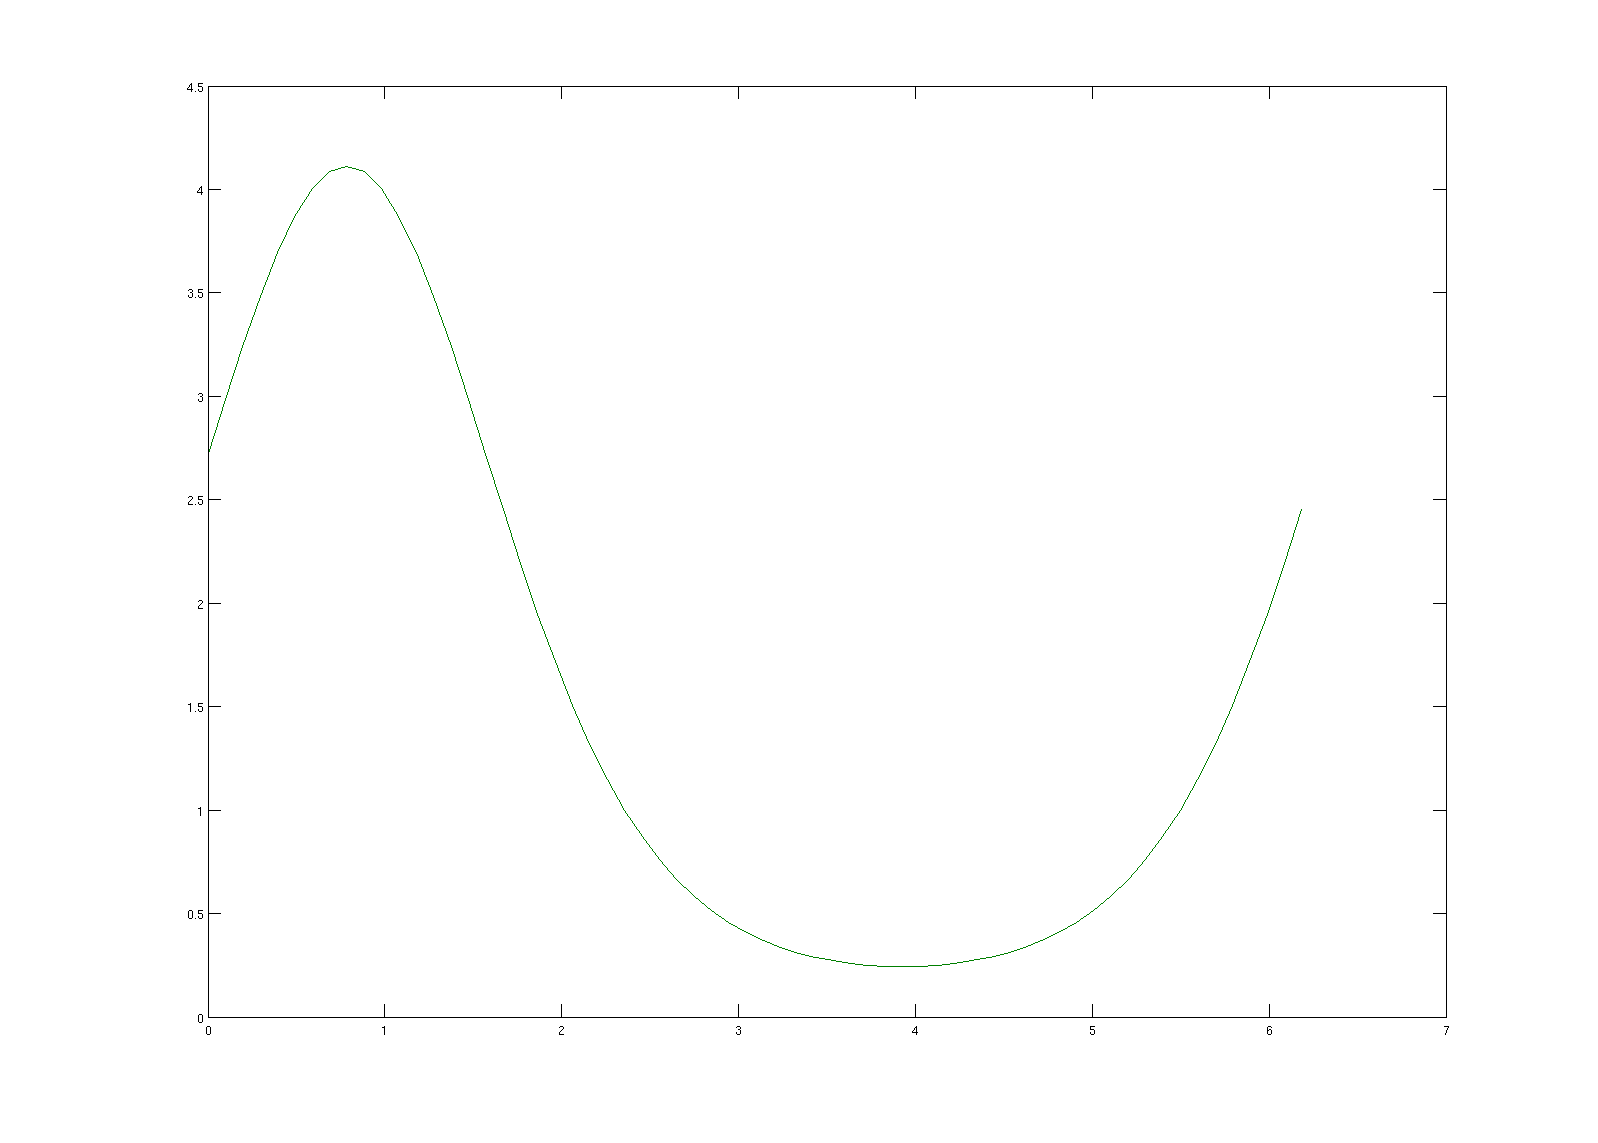
\includegraphics[width=4in]{p1_soln.png}



\paragraph{2} First, observe that the exact solution to this equation is given by:

\sloppy

\begin{eqnarray*}
u(x) & = &   \frac{ e^{-2 x} }
{J_4\left(2 \sqrt{e}\right) Y_4\left(\frac{2}{\sqrt{e}}\right)-J_4\left(\frac{2}{\sqrt{e}}\right) Y_4\left(2 \sqrt{e}\right)} \times \\
& & 
  \left( J_4\left(\frac{2}{\sqrt{e}}\right) \left(24 Y_4\left(2 \sqrt{e} \right)
   J_4\left(2 \sqrt{e^x} \right)-e^2 (;5;-e) Y_4\left(2 \sqrt{e^x} \right) \right) \int_1^{-1} -\frac{1}{24} \pi  e^{2 t} \sin (8 t) Y_4\left(2 \sqrt{e^{t}} \right) \, dt  \right. \\
& + & J_4\left(2 \sqrt{e^x} \right) \left(e^2 (;5;-e) Y_4\left(\frac{2}{\sqrt{e}} \right)-24
   J_4\left(\frac{2}{\sqrt{e}} \right) Y_4\left(2 \sqrt{e} \right) \right) \int_1^x -\frac{1}{24} \pi  e^{2 t} \sin (8 t) Y_4\left(2 \sqrt{e^t} \right) \, dt \\
& + & 2 Y_4\left(\frac{2}{\sqrt{e}} \right) \left(Y_4\left(2 \sqrt{e}\right) J_4\left(2
   \sqrt{e^x}\right)-J_4\left(2 \sqrt{e}\right) Y_4\left(2 \sqrt{e^x}\right)\right) \int_1^{-1} \frac{1}{2} \pi  e^{4 s} \left(;5;-e^{s}\right) \sin (8 s) \, ds \\
& + & \left. 2 Y_4\left(2 \sqrt{e^x}\right) \left(J_4\left(2 \sqrt{e}\right)
   Y_4\left(\frac{2}{\sqrt{e}}\right)-J_4\left(\frac{2}{\sqrt{e}}\right) Y_4\left(2
   \sqrt{e}\right)\right) \int_1^x \frac{1}{2} \pi  e^{4 s} \left(;5;-e^{s}\right) \sin (8 s) \, ds \right)
\end{eqnarray*}
This was computed using mathematica, and is suitably hideous.  The symbols $Y,K$ are Bessel functions and $(;;)$ is the hypergeometric function of the second kind.  A plot of this exact solution in mathematica is as follows:

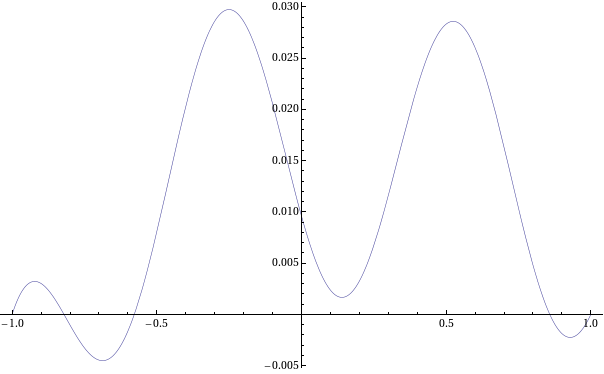
\includegraphics[width=3in]{plot2_mathematica.png}

To solve the system with the Chebyshev method, I used cheb.m, obtained from Nick Trefethen's page and constructed the following solution procedure:

\begin{verbatim}
  [D,x] = cheb(N);        
  D0 = diag(exp(x(2:N)));
  D1 = 4. * D(2:N,2:N);
  D2 = D^2;              
  D2 = D2(2:N,2:N);
  f = sin(8. * x(2:N));
  
  L = D2 + D1 + D0;  
  u = L\f;
  u = [0;u;0];
\end{verbatim}            
  
Here is a plot of my solution:

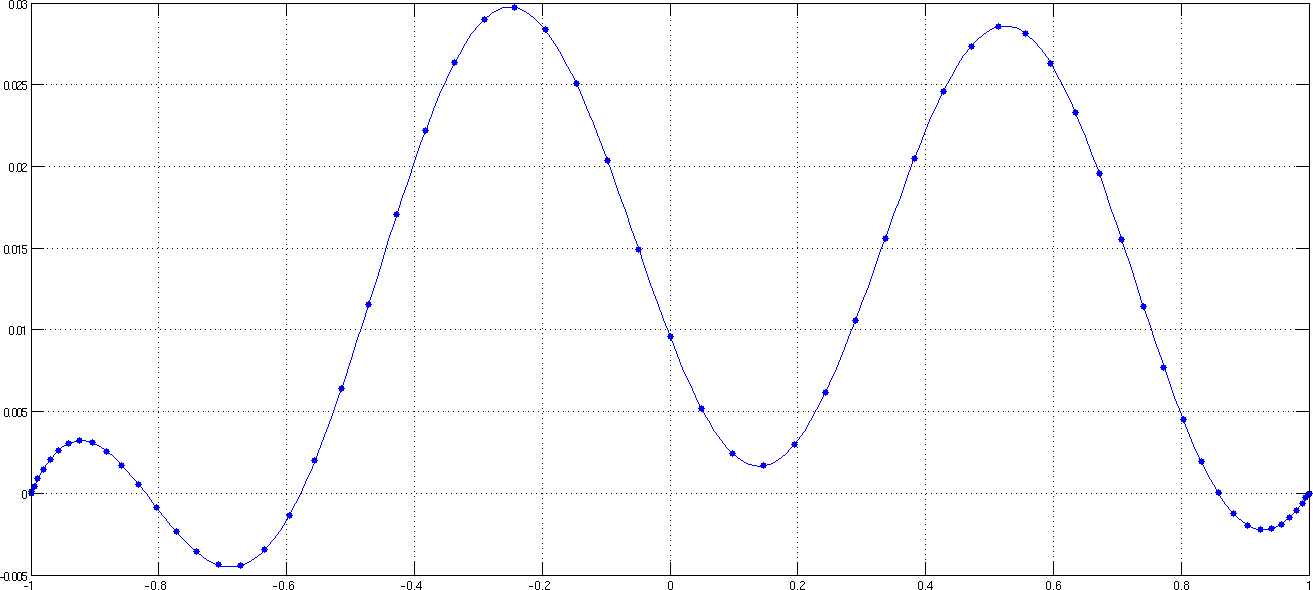
\includegraphics[width=3in]{plot2_matlab.png}

I found that $L^\infty$ error stabilized to 5e-10 around $N \approx 32$.

\paragraph{3}

\subparagraph{a}

Assume that $\sigma(x) > 0$ for all $x \in [0,1]$, (otherwise the solution could be potentially imaginary or undetermined, and so it would be impossible to directly apply Sturm-Liouville theory).  From the boundary condition, we know that $\varphi(1) = 0$.  Combined with the asymptotic solution for the eigenmodes, we get the following equation for $\lambda$:
\[ 0 = \sigma(1)^{-\frac{1}{4}} \sin \left( \sqrt{ \lambda } \int \limits_0^1 \sqrt{ \sigma(\xi) } d \xi \right) \]
Which is true if and only if $\sin(...) = 0$, and so it must be that $... = 0, \pi, 2\pi, ... k \pi$ for all $k \in \mathbb{Z}$.  Thus:
\[ \sqrt{\lambda} \int \limits_0^1 \sqrt{\sigma(\xi)} d \xi = k \pi \]
And so
\[ \lambda \approx \left( \frac{k \pi}{ \int \limits_0^1 \sqrt{ \sigma(\xi) } d \xi } \right) ^2 \]

\subparagraph{b}

This equation may be rewritten as the eigenvalue problem:
\[ \frac{1}{\sigma(x)} \varphi_{xx} = \lambda \varphi \]
To solve this, we again use the cheb.m code from Nick Trefethen.  Here is my MATLAB code:
\begin{verbatim}
  [D,x] = cheb(N);
  D = 2. * D;
  x = .5 * (x + 1);
  sigma = 1. + x;
  D2 = D^2; 
  D2 = D2(2:N,2:N);
  L = diag( 1 ./ sigma(2:N) ) * D2; 
  [V,Lam] = eig(L); 
\end{verbatim}

Substituting $\sigma(x) = 1 + x$, we get $\int \limits_0^1 \sqrt{1 + x} dx = \frac{2}{3} (2 \sqrt{2} - 1 )$ and so:
\[ \lambda \approx \frac{9 \pi ^2 k^2}{4 \left(2 \sqrt{2}-1\right)^2} \]
The first 7 eigen values vs. asymptotic approximation:

\begin{tabular}{cc}
Computed & Estimate \\
    6.5484 & 6.6424 \\
   26.4649 & 26.5697 \\
   59.6742 & 59.7818 \\
  106.1700 & 106.2788 \\
  165.9513 & 166.0607 \\
  239.0177 & 239.1275 \\
  325.3691 & 325.4790
\end{tabular}

Which is reasonably accurate.  Here is a plot of the first 4 eigenvectors:

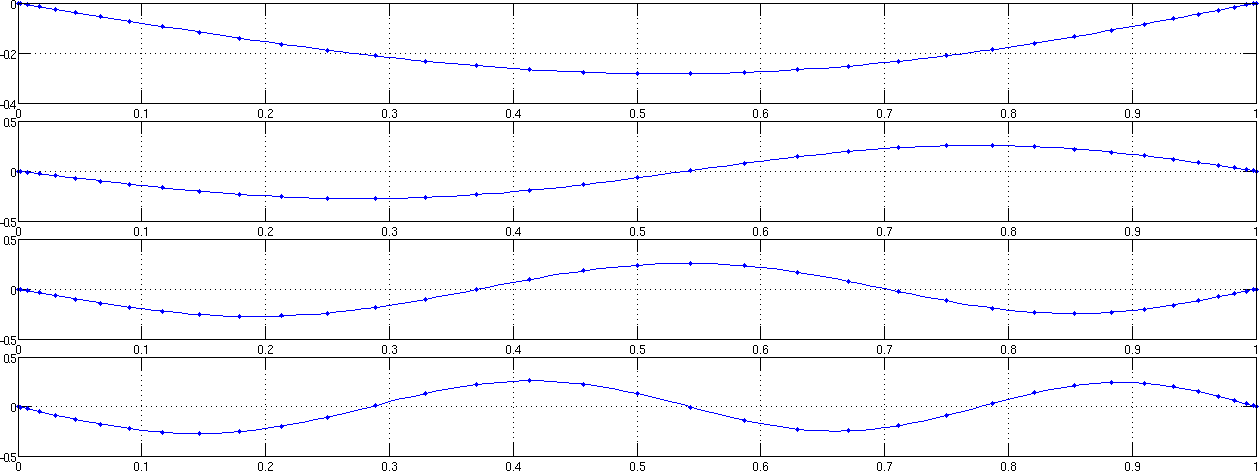
\includegraphics[width=5in]{plot3.png}

\paragraph{4}

\subparagraph{a}

Given that this program solves the BVP given by:
\[ u_{xx} = e^u \] 
Subject to the BCs $u(-1)=u(1)=0$ via the numerical method:
\[ D2 * v_{k+1}  =  \exp(v_{k}) \]
(Where $D2$ is the second order Chebyshev differentiation matrix).  Thus, the $L^\infty$ difference between successive terms is:
\[ | v_{k+1} - v_{k} |_\infty = | D2^{-1} \exp(v_k) - v_k |_\infty \]
Let $\lambda_{max}$ be the magnitude of the largest eigenvalue of $D2^{-1}$, and $V$ be its eigen vector.  Then this quantity is maximized by the choice $v_k = \log(V)$, which gives the asymptotic estimate:
\[ | v_{k+1} - v_{k} |_\infty \approx \lambda_{max}  - \log(\lambda_{max}) \]
The ratio of convergence is given by:
\[ \Delta = \frac{ |v_{k+2} - v_{k+1}|_\infty } { |v_{k+1} - v_{k}|_\infty } = 2 \frac{ | D2^{-1} \exp( D2^{-1} \exp(v_k) - v_k ) - D2^{-1} \exp(v_k) + v_k |_\infty }{ |v_{k+1} - v_{k}|_\infty } \]
Again, we take the eigenvalue expansion and obtain our final approximation for $\Delta$:
\[ \Delta \approx 2 \frac{ \lambda_{max} \exp( \lambda_{max} - \log(\lambda_{max})) - \lambda_{max} + \log( \lambda_{max}) } { \lambda_{max} - \log(\lambda_{max}) } \]
We now evaluate our estimate for $\Delta$ numerically using the following MATLAB code:

\begin{verbatim}
  [v,lam] = eigs(inv(D2))
  lmax = abs(lam(1))
  delta =  2 * (lmax * exp(lmax - log(lmax)) - lmax + log(lmax)) / (lmax - log(lmax))
\end{verbatim}  

Which gives the value $\Delta \approx .2924$.

\subparagraph{b}

We begin by rewriting $u_{xx} = e^u$ as a functional equation:
\[ f(u) = u_{xx} - e^u \]
Which is discretized using the Chebyshev method to give:
\[ f(v) = D2 v - \exp(v) \]
Which has the first variation:
\[ f'(v) = D2 - \Lambda_{\exp(v)} \]
Where $\Lambda_{\exp(v)}$ is a diagonal matrix with values $\exp(v)$.  Thus the Newton's method solution for $k^{th}$ iterate is:
\[ v_{k+1} = v_{k} - \frac{f(v_k)}{f'(v_{k})} \]
Which we compute using the following MATLAB snippet:
\begin{verbatim}
    f = D2 * u - exp(u);
    df = D2  - diag(exp(u));
    unew = u - df \ f;
\end{verbatim}
Unlike the fixed point method, this converges in 5 iterations, which is consistent with the observation that it ought to be quadratic convergence.

\paragraph{5}

The forward Euler method is stable for values of $\Delta t \approx | \lambda |^{-1}$ where $\lambda$ is the largest eigenvalue of the system.  In this case, since we are dealing with a second-order dispersive system, the largest eigenvalue should be in $O(N^2)$ where $N$ is the number of samples.  So to ensure stability, the timestep should be in $\Delta t \in O(N^{-2})$.

The split timestep integration method is implemented as described, though some work was necessary to figure out the parametric form of $v^{**}$.  From the equation, we have:
\begin{eqnarray*}
v^{**} & = & v^* + \frac{\Delta t}{2} D2 ( v^{*} + v^{**} ) \\
(I - \frac{\Delta t}{2} D2) v^{**} & = & (I + \frac{\Delta t}{2} D2) v^* \\
v^{**} & = & (I - \frac{\Delta t}{2} D2)^{-1} (I + \frac{\Delta t}{2} D2) v^*
\end{eqnarray*}

I implemented the split timestep method as described using the following MATLAB code:

\begin{verbatim}
  [D,x] = cheb(N); 
  D2 = D^2; 
  D2 = D2(2:N,2:N);
  M = inv(eye(N-1) - .5 * delta_t * D2) * (eye(N-1) + .5 * delta_t * D2);
  v = zeros(N-1,1);
  for t = 0:delta_t:t_max
    vs  = M * log( 2. * exp(v) ./ (2. - exp(v) * delta_t) );
  	v = log( 2. * exp(vs) ./ (2. - exp(vs) * delta_t));
  end
\end{verbatim}

From this, I numerically computed $u(0, 3.5) \approx 3.5205$ and that $u(0, 3.5364) \approx 5.0000$.

\end{document}
